\documentclass{article}
\usepackage[parfill]{parskip}
\usepackage[utf8]{inputenc}
\usepackage{amsmath}
\usepackage{amsthm} % for proofs
\usepackage{amssymb}
\usepackage{graphicx}
\usepackage{bm}
\usepackage[toc,page]{appendix}
\graphicspath{ {./images} }

\title{Singluar Value Decomposition (SVD)}
\author{Dávid Iván}

\begin{document}

\maketitle

\tableofcontents

\newpage

\section{SVD without proofs}

Let $X$ be an $n$-by-$m$ matrix, with rank $r \le \text{min}(m,n)$. Then we can write $X$ as the sum of $r$ one-rank matrices:

\begin{equation}
    X = \sum_{i=1}^r \sigma_i (u_iv^T_i)
\end{equation}

where $\sigma_i$ is a singular value, always positive, and we assume they are ordered, i.e., $\sigma_1 \ge \sigma_2 \ge \dots \ge \sigma_r$.

The u-vectors form an orthonormal basis in the column space $R(X)$. The v-vectors form an orthonormal basis in the row space $R(X^T)$.

\section{SVD of a centered data matrix}

Let $X$ be an $N$-by-$p$ data matrix, where each row is a data point. We center the data matrix, so that it has zero mean (the sum of each column is zero).

\begin{figure}[ht]
 \centering
  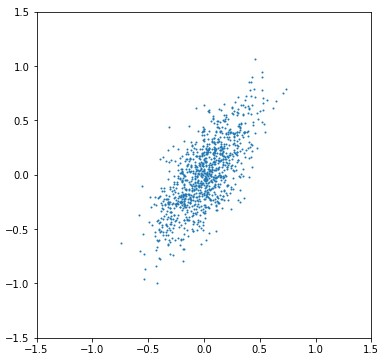
\includegraphics[width=200pt]{images/data_matrix.jpg}
 \caption{Data. The rows of X are thought of as data points.}
\end{figure}

Consider a unit vector (in the row space) $a$. We can project the data points onto $W_a$ (the line defined by $a$) with the projection matrix:

\begin{equation}
    P_a = \frac{aa^T}{a^Ta} = aa^T
\end{equation}

The projection of $v$ onto $W_a$:

\begin{equation}
    v' = P_a v = aa^T v = (a^T v) a
\end{equation}

We see that the projected point is on the line of $a$, and its coordinate (distance from origin) is $a^T v$ (or $v^T a$). We can project all data points, the coordinates are $Xa$. The variance of the data points along the line:

\begin{equation}
    \text{Var}(Xa) = \frac{1}{N} ||Xa||^2
\end{equation}

From this we see that if we want to maximize the variance (finding the first principal direction), $a$ must be $v_1$, and then the variance:

\begin{equation}
    \text{Var}(Xv_1) = \frac{1}{N} ||Xv_1||^2 = \frac{1}{N} ||\sigma_1 u_1||^2 = \frac{\sigma_1^2}{N}
\end{equation}


\begin{figure}[ht]
 \centering
  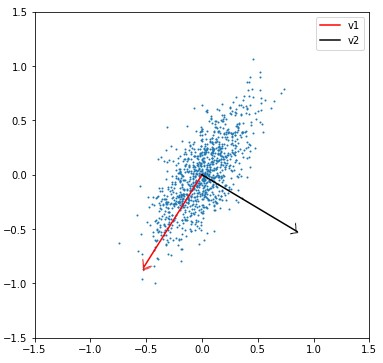
\includegraphics[width=200pt]{images/data_matrix_pca.jpg}
 \caption{SVD of the data matrix. $v_1$ is pointing to the largest variance, $v_2$ is orthogonal to it.}
\end{figure}

So the diagonal form of the covariance matrix is $D^2/N$. The sample covariance:

\begin{equation}
    S = \frac1N X^TX = \frac1N VD^2V^T = V \frac{D^2}{N} V^T
\end{equation}

\newpage
\section{Image compression}

Considering an image as a matrix $A$ ($H$-by-$W$), the SVD gives a possibility to compress the image by considering the most relevant contributions, i.e. those that have the biggest singular values.

\begin{equation}
    A = \sum_{i=1}^{r} \sigma_i \cdot u_i \cdot v^T_i \quad \to \quad \hat{A} = \sum_{i=1}^{c} \sigma_i \cdot u_i \cdot v^T_i
\end{equation}

where $c << r$ is the number of components to consider in the new sum. The following figure shows an example of how it performs.

\begin{figure}[ht]
 \centering
  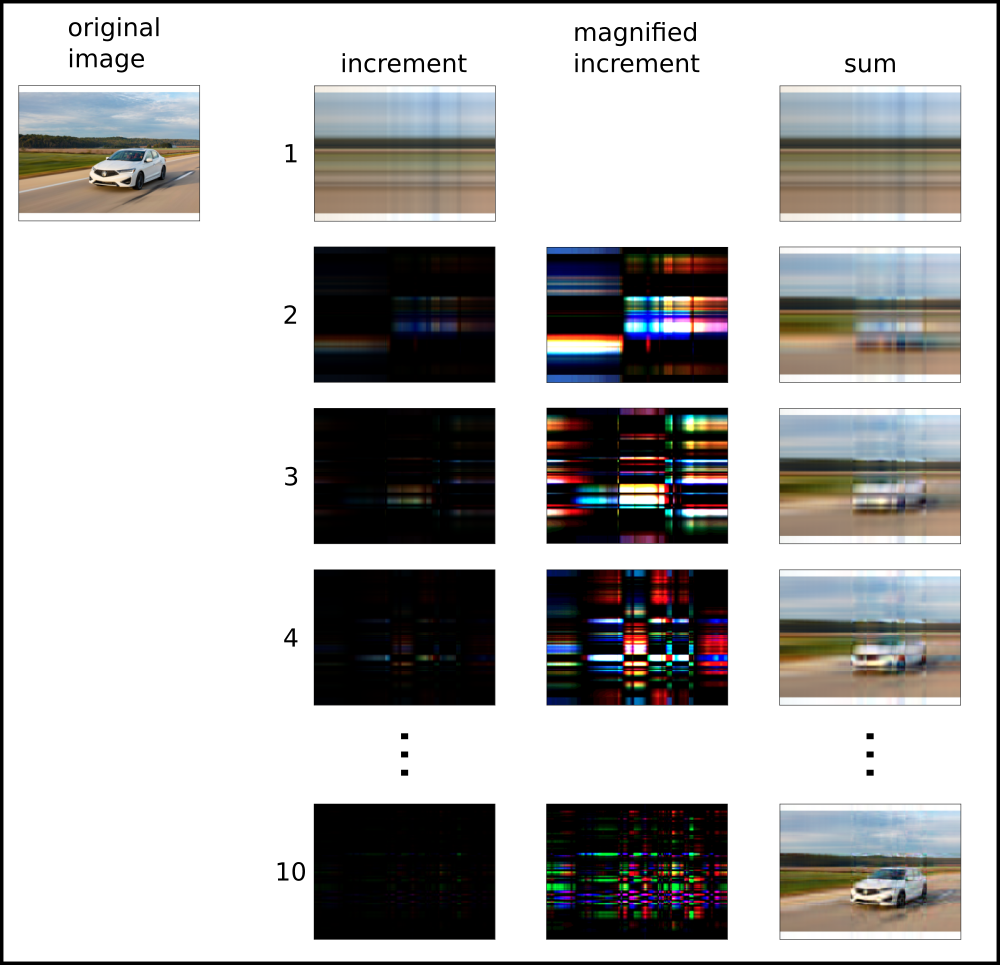
\includegraphics[width=300pt]{images/img_compression.png}
 \caption{Image compression with SVD. Color channels are treated as independent matrices. Here the rank of the (let's say the red) matrix is $r\approx 656$. Taking the first 10 components gives a pretty nice result.}
\end{figure}

\end{document}
